\documentclass[11pt]{article}
\usepackage[margin=1in]{geometry}
\usepackage{graphicx}
\usepackage{amsmath}

\title{\vspace{100pt} E102 Midterm Project \vspace{20pt}}
\author{Kyle Lund, Jesse Joseph, and Josh Sealand}

\begin{document}
\maketitle
\pagebreak

\section*{Introduction}


\section*{Analysis of the Plant}
The plant that we are trying to control is the circuit depicted in figure \ref{fig:circuit}.
This is a simple single input, single output system.

\begin{figure}[h]
\centering
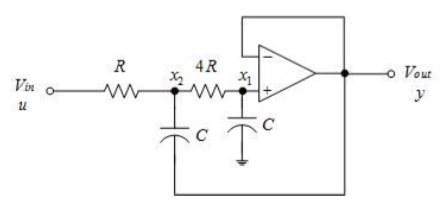
\includegraphics[width=0.6\linewidth]{circuit}
\caption{The circuit schematic for our plant. $C = 10\mu F$ and $R=50k\Omega$}
\label{fig:circuit}
\end{figure}

Immediately, we notice that $y=x_1$, because the $+$ and $-$ terminals of the op-amp must be at approximately equal potential.
This means that our output equation is:

\begin{equation}
y = \begin{bmatrix}
1 & 0
\end{bmatrix}
\begin{bmatrix}
x_1 \\ x_2
\end{bmatrix}
\end{equation}

We can use Kirchhoff's Current Law at the two nodes $x_1$ and $x_2$ to determine the rest of the state space equations for this system.

\begin{align}
x_1:&~~~~ \frac{1}{4R}(x_1-x_2) + C\dot{x}_1 = 0 \label{eq:KCL1} \\ 
x_2:&~~~~ \frac{1}{R}(x_2 - u) + \frac{1}{4R}(x_2-x_1) + C(\dot{x}_2-\dot{x}_1) = 0 \label{eq:KCL2}
\end{align}
%
Now if we solve equation \ref{eq:KCL1} for $\dot{x}_1$, we get:
\begin{equation}
\dot{x}_1 = \frac{1}{4RC}(-x_1+x_2)
\end{equation}
%
Solving equation \ref{eq:KCL2} for $\dot{x}_2$ (and plugging in the result above) we get:
%
\begin{equation}
\dot{x}_2 = \dot{x}_1+\frac{1}{4RC}(x_1-x_2)+\frac{1}{RC}(-x_2+u) =\frac{1}{RC}(-x_2+u)
\end{equation}
%
Putting these equations in matrix form, we obtain:
%
\begin{equation}
\begin{bmatrix}
\dot{x}_1 \\ \dot{x}_2
\end{bmatrix} = 
\begin{bmatrix}
\frac{1}{4RC} & -\frac{1}{4RC} \\
0    & -\frac{1}{RC}
\end{bmatrix}
\begin{bmatrix}
x_1 \\ x_2
\end{bmatrix} + 
\begin{bmatrix}
0 \\ \frac{1}{RC}
\end{bmatrix} u
\end{equation}
%
For our system, $\frac{1}{RC} = \frac{1}{50k\Omega*10\mu F} = 2\mathrm{Hz}$.
Using this, our equations become:
%
\begin{equation}
\begin{bmatrix}
\dot{x}_1 \\ \dot{x}_2
\end{bmatrix} = 
\begin{bmatrix}
\frac{1}{2} & -\frac{1}{2} \\
0    & -2
\end{bmatrix}
\begin{bmatrix}
x_1 \\ x_2
\end{bmatrix} + 
\begin{bmatrix}
0 \\ 2
\end{bmatrix} u
\end{equation}
\section*{Designing the Controller}



\section*{Results}



\end{document}